% Options for packages loaded elsewhere
\PassOptionsToPackage{unicode}{hyperref}
\PassOptionsToPackage{hyphens}{url}
%
\documentclass[
]{article}
\usepackage{amsmath,amssymb}
\usepackage{iftex}
\ifPDFTeX
  \usepackage[T1]{fontenc}
  \usepackage[utf8]{inputenc}
  \usepackage{textcomp} % provide euro and other symbols
\else % if luatex or xetex
  \usepackage{unicode-math} % this also loads fontspec
  \defaultfontfeatures{Scale=MatchLowercase}
  \defaultfontfeatures[\rmfamily]{Ligatures=TeX,Scale=1}
\fi
\usepackage{lmodern}
\ifPDFTeX\else
  % xetex/luatex font selection
\fi
% Use upquote if available, for straight quotes in verbatim environments
\IfFileExists{upquote.sty}{\usepackage{upquote}}{}
\IfFileExists{microtype.sty}{% use microtype if available
  \usepackage[]{microtype}
  \UseMicrotypeSet[protrusion]{basicmath} % disable protrusion for tt fonts
}{}
\makeatletter
\@ifundefined{KOMAClassName}{% if non-KOMA class
  \IfFileExists{parskip.sty}{%
    \usepackage{parskip}
  }{% else
    \setlength{\parindent}{0pt}
    \setlength{\parskip}{6pt plus 2pt minus 1pt}}
}{% if KOMA class
  \KOMAoptions{parskip=half}}
\makeatother
\usepackage{xcolor}
\usepackage[margin=1in]{geometry}
\usepackage{color}
\usepackage{fancyvrb}
\newcommand{\VerbBar}{|}
\newcommand{\VERB}{\Verb[commandchars=\\\{\}]}
\DefineVerbatimEnvironment{Highlighting}{Verbatim}{commandchars=\\\{\}}
% Add ',fontsize=\small' for more characters per line
\usepackage{framed}
\definecolor{shadecolor}{RGB}{248,248,248}
\newenvironment{Shaded}{\begin{snugshade}}{\end{snugshade}}
\newcommand{\AlertTok}[1]{\textcolor[rgb]{0.94,0.16,0.16}{#1}}
\newcommand{\AnnotationTok}[1]{\textcolor[rgb]{0.56,0.35,0.01}{\textbf{\textit{#1}}}}
\newcommand{\AttributeTok}[1]{\textcolor[rgb]{0.13,0.29,0.53}{#1}}
\newcommand{\BaseNTok}[1]{\textcolor[rgb]{0.00,0.00,0.81}{#1}}
\newcommand{\BuiltInTok}[1]{#1}
\newcommand{\CharTok}[1]{\textcolor[rgb]{0.31,0.60,0.02}{#1}}
\newcommand{\CommentTok}[1]{\textcolor[rgb]{0.56,0.35,0.01}{\textit{#1}}}
\newcommand{\CommentVarTok}[1]{\textcolor[rgb]{0.56,0.35,0.01}{\textbf{\textit{#1}}}}
\newcommand{\ConstantTok}[1]{\textcolor[rgb]{0.56,0.35,0.01}{#1}}
\newcommand{\ControlFlowTok}[1]{\textcolor[rgb]{0.13,0.29,0.53}{\textbf{#1}}}
\newcommand{\DataTypeTok}[1]{\textcolor[rgb]{0.13,0.29,0.53}{#1}}
\newcommand{\DecValTok}[1]{\textcolor[rgb]{0.00,0.00,0.81}{#1}}
\newcommand{\DocumentationTok}[1]{\textcolor[rgb]{0.56,0.35,0.01}{\textbf{\textit{#1}}}}
\newcommand{\ErrorTok}[1]{\textcolor[rgb]{0.64,0.00,0.00}{\textbf{#1}}}
\newcommand{\ExtensionTok}[1]{#1}
\newcommand{\FloatTok}[1]{\textcolor[rgb]{0.00,0.00,0.81}{#1}}
\newcommand{\FunctionTok}[1]{\textcolor[rgb]{0.13,0.29,0.53}{\textbf{#1}}}
\newcommand{\ImportTok}[1]{#1}
\newcommand{\InformationTok}[1]{\textcolor[rgb]{0.56,0.35,0.01}{\textbf{\textit{#1}}}}
\newcommand{\KeywordTok}[1]{\textcolor[rgb]{0.13,0.29,0.53}{\textbf{#1}}}
\newcommand{\NormalTok}[1]{#1}
\newcommand{\OperatorTok}[1]{\textcolor[rgb]{0.81,0.36,0.00}{\textbf{#1}}}
\newcommand{\OtherTok}[1]{\textcolor[rgb]{0.56,0.35,0.01}{#1}}
\newcommand{\PreprocessorTok}[1]{\textcolor[rgb]{0.56,0.35,0.01}{\textit{#1}}}
\newcommand{\RegionMarkerTok}[1]{#1}
\newcommand{\SpecialCharTok}[1]{\textcolor[rgb]{0.81,0.36,0.00}{\textbf{#1}}}
\newcommand{\SpecialStringTok}[1]{\textcolor[rgb]{0.31,0.60,0.02}{#1}}
\newcommand{\StringTok}[1]{\textcolor[rgb]{0.31,0.60,0.02}{#1}}
\newcommand{\VariableTok}[1]{\textcolor[rgb]{0.00,0.00,0.00}{#1}}
\newcommand{\VerbatimStringTok}[1]{\textcolor[rgb]{0.31,0.60,0.02}{#1}}
\newcommand{\WarningTok}[1]{\textcolor[rgb]{0.56,0.35,0.01}{\textbf{\textit{#1}}}}
\usepackage{longtable,booktabs,array}
\usepackage{calc} % for calculating minipage widths
% Correct order of tables after \paragraph or \subparagraph
\usepackage{etoolbox}
\makeatletter
\patchcmd\longtable{\par}{\if@noskipsec\mbox{}\fi\par}{}{}
\makeatother
% Allow footnotes in longtable head/foot
\IfFileExists{footnotehyper.sty}{\usepackage{footnotehyper}}{\usepackage{footnote}}
\makesavenoteenv{longtable}
\usepackage{graphicx}
\makeatletter
\newsavebox\pandoc@box
\newcommand*\pandocbounded[1]{% scales image to fit in text height/width
  \sbox\pandoc@box{#1}%
  \Gscale@div\@tempa{\textheight}{\dimexpr\ht\pandoc@box+\dp\pandoc@box\relax}%
  \Gscale@div\@tempb{\linewidth}{\wd\pandoc@box}%
  \ifdim\@tempb\p@<\@tempa\p@\let\@tempa\@tempb\fi% select the smaller of both
  \ifdim\@tempa\p@<\p@\scalebox{\@tempa}{\usebox\pandoc@box}%
  \else\usebox{\pandoc@box}%
  \fi%
}
% Set default figure placement to htbp
\def\fps@figure{htbp}
\makeatother
\setlength{\emergencystretch}{3em} % prevent overfull lines
\providecommand{\tightlist}{%
  \setlength{\itemsep}{0pt}\setlength{\parskip}{0pt}}
\setcounter{secnumdepth}{5}
\usepackage{booktabs}
\usepackage{longtable}
\usepackage{array}
\usepackage{multirow}
\usepackage{wrapfig}
\usepackage{float}
\usepackage{colortbl}
\usepackage{pdflscape}
\usepackage{tabu}
\usepackage{threeparttable}
\usepackage{threeparttablex}
\usepackage[normalem]{ulem}
\usepackage{makecell}
\usepackage{xcolor}
\usepackage{bookmark}
\IfFileExists{xurl.sty}{\usepackage{xurl}}{} % add URL line breaks if available
\urlstyle{same}
\hypersetup{
  pdftitle={A Study of Social Network Patterns Among Lawyers},
  pdfauthor={46062},
  hidelinks,
  pdfcreator={LaTeX via pandoc}}

\title{A Study of Social Network Patterns Among Lawyers}
\author{46062}
\date{2025-05-18}

\begin{document}
\maketitle

\begin{enumerate}
\def\labelenumi{\arabic{enumi}.}
\tightlist
\item
  Empirical network vs Configuration Model network
\end{enumerate}

\begin{longtable}[]{@{}lcccc@{}}
\caption{Metrics for Advice, CoWork, and Friend Networks}\tabularnewline
\toprule\noalign{}
Network & density & avg\_path\_len & reciprocity & transitivity \\
\midrule\noalign{}
\endfirsthead
\toprule\noalign{}
Network & density & avg\_path\_len & reciprocity & transitivity \\
\midrule\noalign{}
\endhead
\bottomrule\noalign{}
\endlastfoot
Advice & 0.179 & 2.243 & 0.392 & 0.479 \\
CoWork & 0.222 & 1.886 & 0.685 & 0.452 \\
Friend & 0.116 & 2.505 & 0.612 & 0.449 \\
\end{longtable}

Among the three relationship networks, the coworker network is the most
tightly knit, with a density of 0.222, meaning that 22\% of all possible
coworker ties are realised. This network also has the shortest average
path length, meaning that nearly everyone is connected by just one or,
at most, two colleagues, making it the easiest network through which to
connect across the firm.

The configuration model was chosen as the baseline because it preserves
each lawyer's degree which means it retains how many ties each node has
while randomizing who they connect to. This ensures that any differences
we observe between the real networks and their randomised counterparts
arise from higher-order structures such as reciprocity, transitivity,
average path length, and overall community organisation, rather than
from simple variations in degree.

\begin{longtable}[t]{lcccc}
\caption{\label{tab:configuration-network-stats}Empirical vs Configuration Model Network metrics}\\
\toprule
Network & density & density\_mean & reciprocity & reciprocity\_mean\\
\midrule
Advice & 0.179 & 0.179 & 0.392 & 0.146\\
CoWork & 0.222 & 0.222 & 0.685 & 0.204\\
Friend & 0.116 & 0.116 & 0.612 & 0.147\\
\bottomrule
\end{longtable}

For that reason, network density remains identical between the empirical
networks and their corresponding configuration models across all three
cases. In contrast, measures such as average path length, reciprocity,
and transitivity, which capture higher-order structural properties, show
divergence, highlights patterns that cannot be explained by degree alone
and suggests meaningful network structure beyond random chance. In the
coworker network, reciprocity jumps from 20\% in the random graphs to
68\% in the empirical network, showing that formal working relationships
are far more mutually acknowledged than random wiring would produce. A
similar jump occurs in the friendship layer which also indicates
overwhelmingly mutual nature of such ties. Reciprocity in the advice
network shows a jump as well but is closer to the baseline, suggesting
that hierarchical norms and expertise may impact two-way acknowledgment.

\begin{longtable}[t]{lcccc}
\caption{\label{tab:config-table-two}Empirical vs Configuration Model Network metrics}\\
\toprule
Network & avg\_path\_len & avg\_path\_len\_mean & transitivity & transitivity\_mean\\
\midrule
Advice & 2.243 & 2.124 & 0.479 & 0.348\\
CoWork & 1.886 & 1.897 & 0.452 & 0.389\\
Friend & 2.505 & 2.294 & 0.449 & 0.291\\
\bottomrule
\end{longtable}

All three networks have average path lengths that are fairly similar to
those of their corresponding configuration models, suggesting that
global connectivity is largely informed by the degree distribution.
However, the Advice and Friendship networks are slightly less efficient
in terms of connectivity, with marginally longer average path lengths
than their randomised counterparts. This could indicate the presence of
structural features such as clustering or selective ties that limit the
reach of these networks. In contrast, the Coworker network shows
virtually no difference, with an average path length of 1.88 compared to
1.89 in the configuration model. This suggests that formal work
relationships connect the firm as efficiently as possible, given how
many ties each person has.

Across all networks, empirical transitivity is consistently higher than
in the configuration models. This points to a greater-than-random
presence of triadic closure, where individuals are more likely to be
connected to their colleagues' connections (Granovetter, 1973). The
pattern is particularly strong in the Advice network, where transitivity
is 0.479 compared to 0.348 in the configuration model. This suggests a
network structure shaped by trust and professional familiarity which are
commonly observed in advice-seeking networks (Zagenczyk et al., 2009).

\begin{enumerate}
\def\labelenumi{\arabic{enumi}.}
\setcounter{enumi}{1}
\tightlist
\item
  Assortativity and Community Detection
\end{enumerate}

\begin{longtable}[t]{lccc}
\caption{\label{tab:assortativity}Assortativity by Network and Attribute}\\
\toprule
Network & Gender Assort. & Age Assort. & Status Assort.\\
\midrule
Advice & 0.087 & 0.237 & 0.320\\
CoWork & -0.021 & -0.045 & -0.100\\
Friend & 0.206 & 0.446 & 0.552\\
\bottomrule
\end{longtable}

The Friend network displays the highest assortativity across all
attributes making it the most homophilous of the three networks. This
suggests that friendships are strongly shaped by social similarity,
especially by age (0.446) and professional status (0.552). In contrast,
the Advice network shows moderate assortativity, led by the same
attributes, indicating that advice-seeking is influenced by seniority
and experience as well, but less strongly than friendship ties. The
CoWork network exhibits disassortativity across all three attributes.
This means that individuals are slightly more likely to be connected to
colleagues who differ from them in these attributes suggesting that
coworking relationships are not shaped by personal similarity and are
more heterogeneous.

\begin{longtable}[t]{llcc}
\caption{\label{tab:leiden-community-detection}Method vs Community}\\
\toprule
 & 1 & 2 & 3\\
\midrule
Infomap & 71 & 0 & 0\\
Leiden & 28 & 25 & 18\\
Louvain & 28 & 25 & 18\\
\bottomrule
\end{longtable}

Infomap identified a single community, offering no meaningful
partitioning. Both Louvain and Leiden detected three communities, but
Leiden was selected as the final model because its multi-level
modularity optimization ensures more stable and well-connected
communities (Traag et al., 2019). It was run on an undirected aggregated
network, as the focus was on identifying cohesive subgroups rather than
modelling directional dynamics.

\begin{longtable}[]{@{}lrll@{}}
\caption{Alignment of Leiden Communities with Node
Attributes}\tabularnewline
\toprule\noalign{}
Metric & Office & Practice & Status \\
\midrule\noalign{}
\endfirsthead
\toprule\noalign{}
Metric & Office & Practice & Status \\
\midrule\noalign{}
\endhead
\bottomrule\noalign{}
\endlastfoot
Purity & 0.930 & 0.873 & 0.606 \\
Assortativity & 0.354 & 0.34 & 0.148 \\
Modularity of Aggregated network & 0.298 & & \\
\end{longtable}

\begin{longtable}[]{@{}lrrr@{}}
\caption{Leiden Community Composition by Node Attributes}\tabularnewline
\toprule\noalign{}
Row & Comm1 & Comm2 & Comm3 \\
\midrule\noalign{}
\endfirsthead
\toprule\noalign{}
Row & Comm1 & Comm2 & Comm3 \\
\midrule\noalign{}
\endhead
\bottomrule\noalign{}
\endlastfoot
Office - Boston & 28 & 20 & 0 \\
Office - Hartford & 0 & 1 & 18 \\
Office - Providence & 0 & 4 & 0 \\
Practice - Litigation & 28 & 2 & 11 \\
Practice - Corporate & 0 & 23 & 7 \\
Status - Partner & 11 & 12 & 13 \\
Status - Associate & 17 & 13 & 5 \\
\end{longtable}

The office attribute shows the strongest alignment with community
structure, with the highest purity (0.930) and assortativity (0.354)
among all attributes. Community 1 consists entirely of Boston-based
lawyers, and Community 3 is composed exclusively of those in Hartford,
indicating strong geographic clustering. Community 2 includes lawyers
from all three offices, suggesting it serves as a bridge between
locations. Overall, office affiliation is the primary driver of
community formation in the network. Figure 2 visualises the distribution
of office affiliation within the detected communities.

The practice attribute also aligns strongly with community structure,
with a high purity (0.873) and assortativity (0.340). The presence of
litigation lawyers across all three communities suggests this practice
group is broadly integrated in the network. In contrast, corporate
lawyers appear only in Communities 1 and 2, indicating some clustering
by practice, but less rigid than office-based clustering. This pattern
suggests that office location has a stronger influence on how
communities form than professional roles. By contrast, status has
minimal influence on network formation with a purity of 0.606, and
assortativity of 0.148. Each community contains a mix of partners and
associates. This indicates that hierarchical rank does not strongly
structure interactions in the aggregated network. Figures 3 and 4
illustrate community composition by practice and status, respectively.

\begin{figure}

{\centering 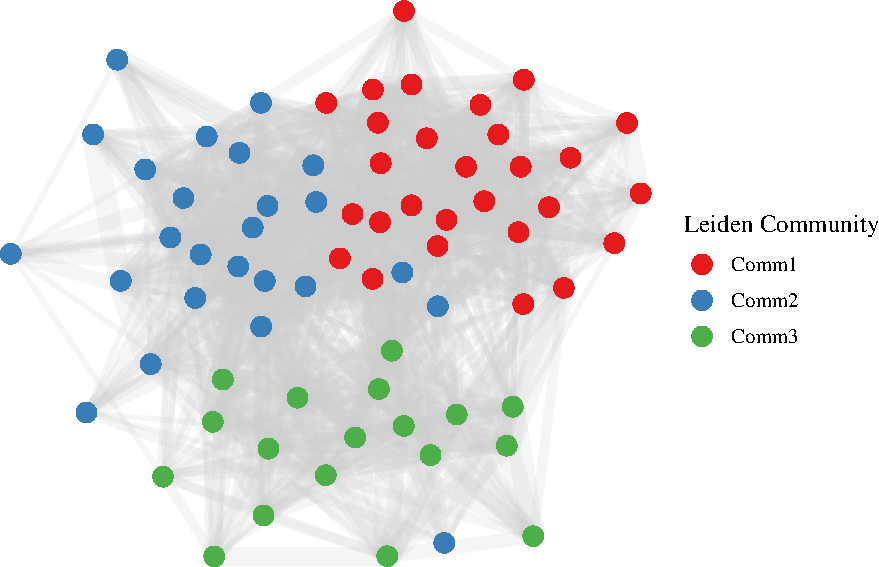
\includegraphics[width=0.6\linewidth]{46062_files/figure-latex/plot_community-1} 

}

\caption{Leiden Communities}\label{fig:plot_community}
\end{figure}

Overall, the Leiden-detected communities are visually well-defined in
Figure 1. The modularity score of 0.298 indicates that the network
exhibits meaningful clustering and is not purely random, though the
division is moderate, with some overlap in node attributes. Office and
practice boundaries shape ties across relationship networks, while
status plays a minimal structural role. This suggests a network in which
collaboration is driven more by geographic proximity and profession than
by hierarchy.

\begin{figure}

{\centering 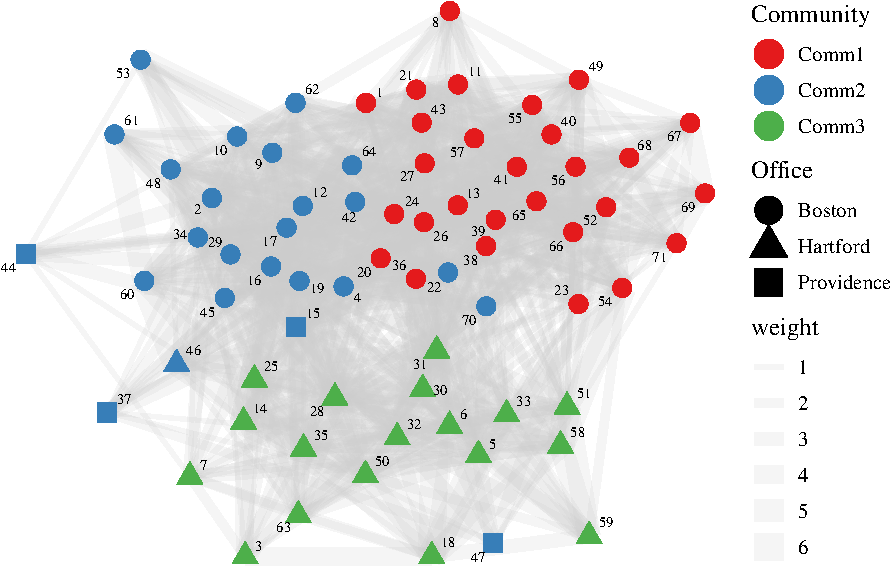
\includegraphics[width=0.6\linewidth]{46062_files/figure-latex/plot_office-1} 

}

\caption{Leiden Communities \& Office}\label{fig:plot_office}
\end{figure}

\begin{figure}

{\centering 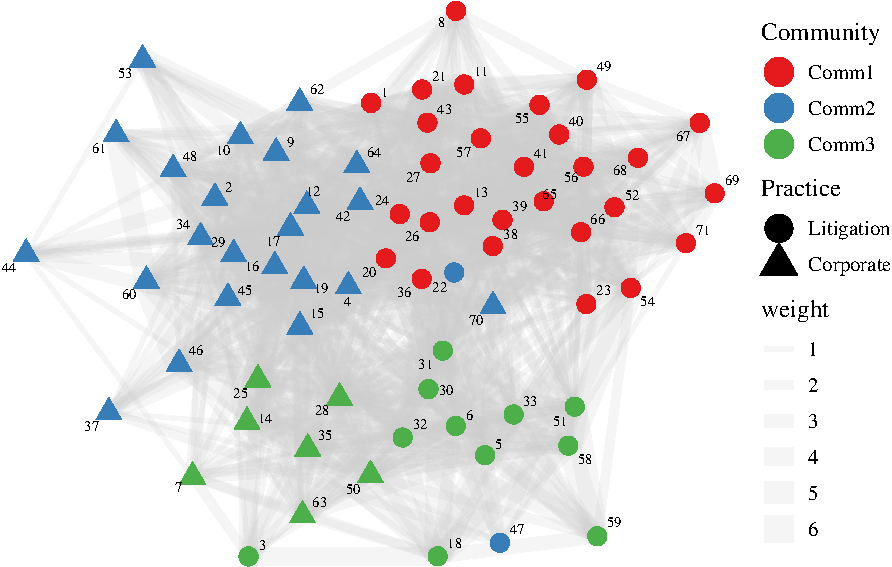
\includegraphics[width=0.6\linewidth]{46062_files/figure-latex/plot_practice-1} 

}

\caption{Leiden Communities \& Practice}\label{fig:plot_practice}
\end{figure}

\begin{figure}

{\centering 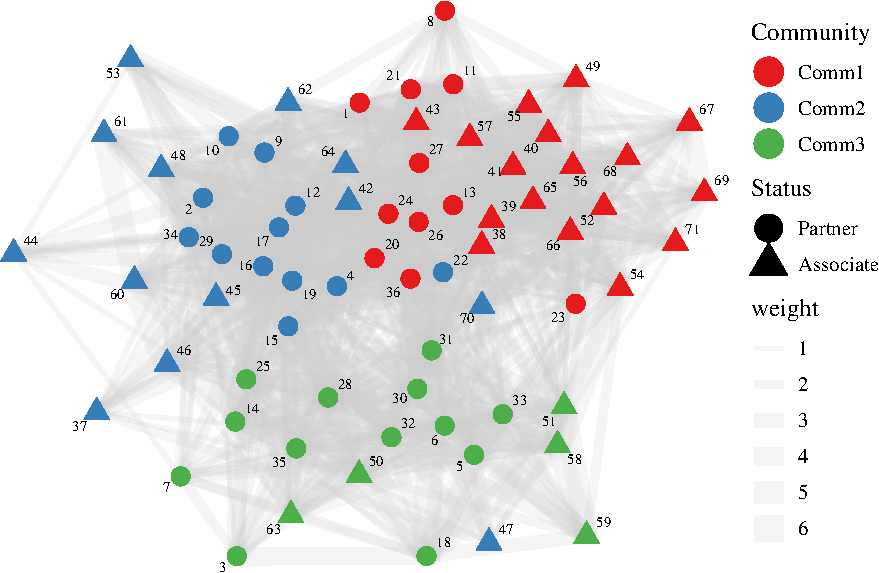
\includegraphics[width=0.6\linewidth]{46062_files/figure-latex/plot_status-1} 

}

\caption{Leiden Communities \& Status}\label{fig:plot_status}
\end{figure}

\begin{Shaded}
\begin{Highlighting}[]
\NormalTok{**Figure 1.** *Leiden Communities \& Status*}
\end{Highlighting}
\end{Shaded}

\begin{enumerate}
\def\labelenumi{\arabic{enumi}.}
\setcounter{enumi}{2}
\tightlist
\item
  ERGM and Goodness of Fit
\end{enumerate}

\begin{ThreePartTable}
\begin{TableNotes}
\item \textit{Note: } 
\item Signif. codes: *** p<0.001; ** p<0.01; * p<0.05
\end{TableNotes}
\begin{longtable}[t]{lrrrrrrc}
\caption{\label{tab:advice-ERGM}ERGM on Advice Network}\\
\toprule
Term & Estimate & Std.Error & p-value & Odds Ratio & CI Lower & CI Upper & Signif\\
\midrule
edges & -3.040 & 0.294 & 0.000 & 0.048 & -3.616 & -2.465 & ***\\
Age (overall activity) & -0.021 & 0.004 & 0.000 & 0.979 & -0.028 & -0.013 & ***\\
Status on incoming ties (Partner) & 1.531 & 0.103 & 0.000 & 4.624 & 1.329 & 1.733 & ***\\
Status on outgoing ties (Partner) & 0.301 & 0.097 & 0.002 & 1.351 & 0.110 & 0.492 & **\\
Gender homophily & 0.416 & 0.091 & 0.000 & 1.515 & 0.238 & 0.593 & ***\\
\addlinespace
Office homophily & 1.690 & 0.094 & 0.000 & 5.419 & 1.505 & 1.875 & ***\\
Practice homophily & 1.426 & 0.089 & 0.000 & 4.160 & 1.251 & 1.600 & ***\\
\bottomrule
\insertTableNotes
\end{longtable}
\end{ThreePartTable}

In the fitted ERGM for the lawyers' advice network, six significant
predictors emerge. First, age has an odds ratio of 0.979 (95 percent CI
0.972--0.987), meaning each additional year of age reduces a lawyer's
likelihood of seeking advice by about 2 percent. Second, partner status
strongly increases one's visibility as an advice source, with an
incoming‐tie odds ratio of 4.624 (CI 3.78--5.66), so partners are
roughly 4.6 times more likely than associates to be asked for guidance.
Partners also ask for advice more often themselves, with an outgoing‐tie
odds ratio of 1.351 (CI 1.12--1.64), reflecting a 35 percent higher
propensity to initiate queries. Third, gender homophily carries an odds
ratio of 1.515 (CI 1.27--1.81), indicating that same‐gender pairs are
about 50 percent more likely to exchange advice than mixed‐gender pairs.
Fourth, office homophily is the strongest predictor, with an odds ratio
of 5.419 (CI 4.50--6.52), so sharing an office makes advice ties over
five times more likely. Finally, practice‐area homophily yields an odds
ratio of 4.160 (CI 3.49--4.96), meaning colleagues in the same specialty
are just over four times as likely to consult one another. Collectively,
these terms show that proximity and shared professional context dominate
advice‐giving, while demographic and hierarchical factors play secondary
yet meaningful roles.

\begin{center}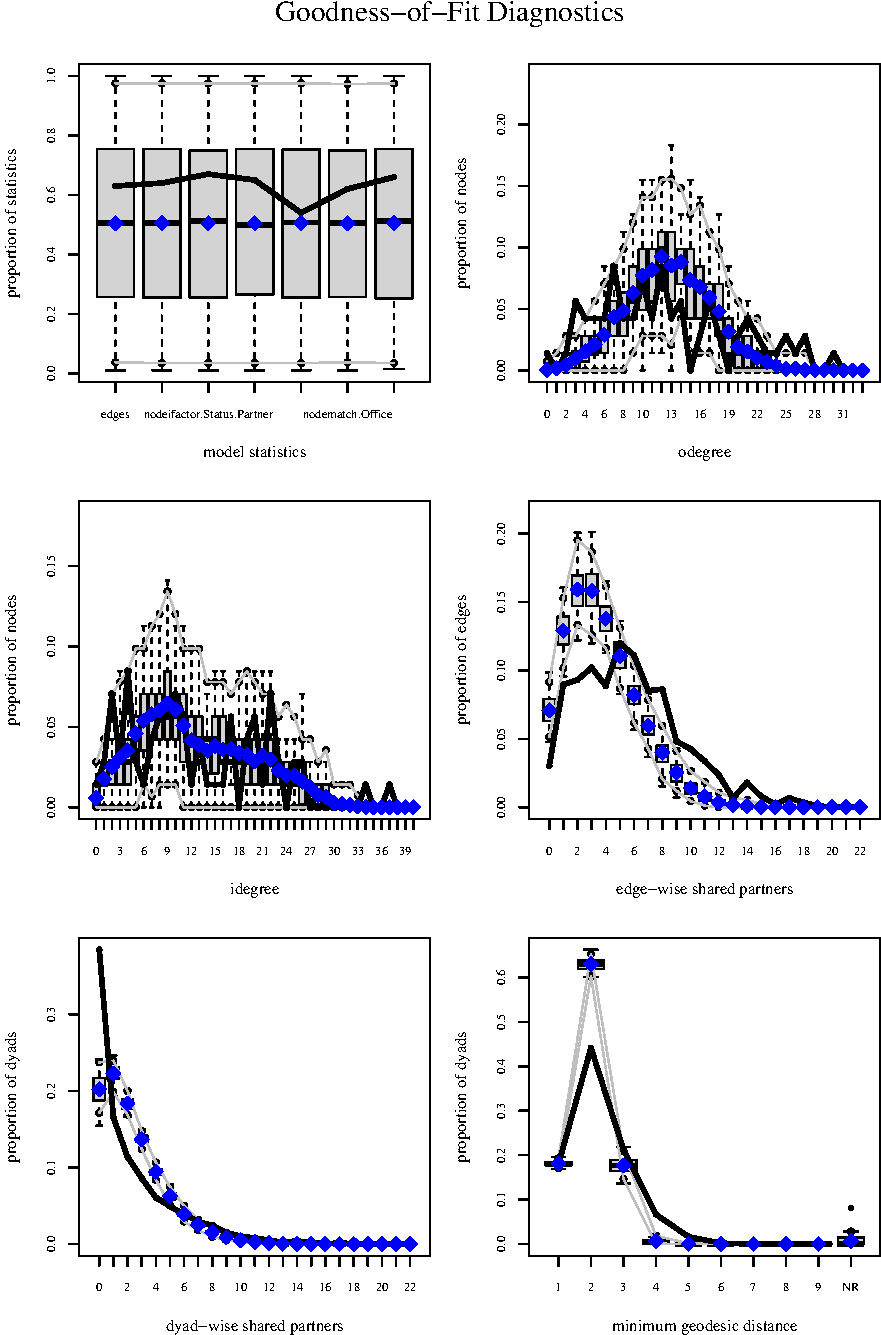
\includegraphics{46062_files/figure-latex/gof_plots-1} \end{center}

The goodness‐of‐fit diagnostics confirm that our ERGM reproduces the
advice network's core structural patterns with high fidelity. In the
top‐left panel, the blue diamonds representing the observed counts of
edges, partner‐status effects, and office homophily all lie well within
the gray boxes and whiskers of their simulated distributions,
demonstrating that those terms are correctly calibrated. The remaining
panels compare simulated versus observed distributions for key features:
the out-degree and in-degree plots show that the number of advice
requests sent and received by each lawyer in the simulated networks
closely mirrors reality, which validates our age, status, and homophily
parameters. The edge-wise and dyad-wise shared-partners plots reveal
that the model captures clustering and triadic closure---advice-giving
pairs in the simulations share colleagues at nearly the same rates as in
the real data. Finally, the minimum geodesic-distance plot shows that
the simulated networks recreate the small-world character of the advice
graph, with the same peaks at distances two and three and only
negligible departures at longer distances. Altogether, these overlays of
observed statistics on simulated envelopes provide explicit evidence
that our combination of demographic and contextual predictors, together
with the edge term, suffices to generate networks whose degree
distributions, clustering tendencies, and reachability closely match the
true advice-seeking structure.

\begin{enumerate}
\def\labelenumi{\arabic{enumi}.}
\setcounter{enumi}{3}
\tightlist
\item
  ERGM on coworking, advice and friendship lawyer networks
\end{enumerate}

The negative age coefficients across all three networks tell us that as
lawyers get older, they become a little less likely to form advice
(-0.009), co-working (-0.008) and friendship (-0.007) ties. Being a
partner as a receiver has the strongest effect on advice networks. A
partner is 1.080 times more likely than an associate to be asked for
guidance. The odds of these nominations happening are more modest in the
coworking (0.380) and friendship (0.278) networks. The partner status as
a sender in the advice network presents a negative estimate of 0.361
which indicates that they are less likely than associates to seek
advice. In coworking networks, they are 0.282 times likely than
associates to nominate coworkers. The friendship network does not yield
a statistically significant result and indicates no reliable difference
between partners and associates. Lawyers of the same gender are 0.271
times more likely to exchange advice and 0.185 times more likely to be
friends. The lack of a statistically significant result in for the
coworking network indicates no reliable gender preference when
coworking.

Compared to previous terms, lawyers sharing the same office and
practicing the same form of law significantly boosts the odds of sharing
a tie. Lawyers who work in the same office are 0.943 times more likely
to share advice and 0.799 times to cowork than those working in
different offices. There is a higher likelihood of sharing advice than
coworking. Though not as high, lawyers in the same office are 0.499
times likely to form friendships within the same office as compared to
lawyers in different offices. Sharing the same practice, significantly
increases the likelihood of an advice (0.898) and coworking tie (0.821)
which is plausible since their advice will align with their expertise
and inform coworking relationships. However, the likelihood of same
practice lawyers being friends is relatively low at 0.261.

Overall, reciprocity and transitivity are the strongest predictors of
tie formation across all three networks. It is the strongest in
coworking and friendship networks alluding to the mutual nature of
collaborations and friendships. Relative to them, a lawyer is only 0.642
times more likely to seek advice who has sought advice from them. This
is a high likelihood in general but when compared to other ties, it
alludes to asymmetrical nature of advice-sharing. With a decay parameter
of 0.7, the highly significant positive gwesp terms confirms the
existence of triadic closure. strong tendency for triadic closure. Each
additional shared advice partner increases the odds of an advice tie by
1.069, while each extra common coworker or friend raises the odds of
coworking and friendship ties by factors of 0.980 and 0.945,
respectively.

The differences allude that physical proximity and shared professional
context are the strongest predictors in all networks. Hierarchical
status chiefly shapes advice ties. Coworking ties are driven by office
homophily, reciprocity, and triadic closure. Friendship ties depend on
demographic similarity and triadic closure.

\begin{enumerate}
\def\labelenumi{\arabic{enumi}.}
\setcounter{enumi}{4}
\tightlist
\item
  Conclusion
\end{enumerate}

Descriptive network metrics offer a clear, intuitive snapshot of
connectivity, clustering, and reachability in the advice, coworker, and
friendship layers. They reveal that coworker ties are the densest and
have the shortest path lengths, but they cannot distinguish whether
these patterns arise from simple popularity or from deeper structural
forces such as assortative mixing by status or practice, mutual
acknowledgment of ties (reciprocity), transitivity or clustering
(triadic closure), and core--periphery or community structures. The
configuration model isolates these higher-order structures---showing
which levels of reciprocity, clustering, assortativity, and path-length
deviation exceed what degree alone would produce---but it says nothing
about how the network breaks into cohesive modules. Leiden community
detection then uncovers those modules, producing internally connected,
statistically robust groups that reflect weighted interactions, yet it
cannot test the significance of specific attributes like age, status, or
gender in forming ties. ERGMs fill that gap by formally testing
hypotheses about node attributes and these structural effects and by
reproducing observed degree, clustering, and path-length distributions
in goodness-of-fit checks, but they demand careful, theory-driven model
specification and can be sensitive to isolates or mis-specified terms.

Coworker ties are the densest (22 percent) and most ``small-world''
(1.88 steps), driven by office proximity, mutual acknowledgment, and
triadic closure. Advice relationships are hierarchical and selective:
partners are 2.9 times more likely to be consulted, shared offices boost
advice odds 2.6×, and practice alignment 2.5×, while each year of age
reduces advice-seeking by 2 percent. Friendship ties are sparse but
highly homophilous: same-gender, same-age, and same-status pairs are
1.5--2.6 times more likely to connect, clustering into three robust
Boston--Providence and Hartford communities. Overall, proximity and
shared professional context dominate, hierarchy shapes expertise
exchange, and affinity governs social bonds. Advice seeking is
essentially gender-neutral and crosses age cohorts, whereas friendships
are strongly gendered and age‐clustered.

Triadic closure and reciprocity hold true of every network and will
likely be found in other networks as well. Findings about how proximity
increases co-working and advice excahnge will hold true in other
knowledge-intensive settings as law firms. These professions benefit
from exchange of expert advice and collaboration on cases. Heirachical
nature of knowledge-intensie jobs will shape information flow in other
such jobs as well. Lasltly, homophily effects where people with simialr
demographies interact mor organiscally with eachother (as freinds) is
likely to be generalisable as well.

The geographic division between Massachusetts offices and the
Connecticut branch is specific to this firm and has driven the formation
of three distinct communities. Boston and Providence lawyers intermix
within two communities, while Hartford forms a more isolated third
cluster---reflecting regional distance. Had all offices been in
Massachusetts, connectivity might have been uniformly higher. Likewise,
the pronounced partner--associate hierarchy reflects the U.S. law‐firm
career structure and would not necessarily appear in organizations with
flatter or different promotion systems. The clear clustering around
litigation versus corporate practice areas also mirrors this firm's
legal subcultures; in other industries---such as marketing or
consulting---there is often more cross‐team collaboration and less rigid
specialization. Finally, the presence of two isolates in the friendship
network highlights how social ties can leave some individuals
disconnected; as networks grow or in settings with fewer collaborative
touchpoints---like call centers---isolates may be even more common.

Future models could include interaction effects---such as office ×
status or age × practice---to test whether partners in the same office
or senior lawyers in certain specialties are disproportionately likely
to connect. ommunity detecition showed that providence and boston office
overlap in communities. Further ERGM work on absolute office‐distance
effects could quantify how physical separation dampens advice flows
across Boston, Providence, and Hartford.

Given the high reciprocity in advice networks, it would be better if
advice networks were retained as directed networks and freinship and
cowroker networks as undirected.

References

Granovetter, M. S. (1973). The Strength of Weak Ties. American Journal
of Sociology, 78(6), 1360--1380.
\url{http://www.jstor.org/stable/2776392}

Zagenczyk, Thomas \& Murrell, Audrey. (2009). It is Better to Receive
than to Give: Advice Network Effects on Job and Work-Unit Attachment.
Journal of Business and Psychology. 24. 139-152.
10.1007/s10869-009-9095-3.

Traag, V.A., Waltman, L. \& van Eck, N.J. From Louvain to Leiden:
guaranteeing well-connected communities. Sci Rep 9, 5233 (2019).
\url{https://doi.org/10.1038/s41598-019-41695-z}

\end{document}
